\documentclass[29pt,a4paper]{moderncv}

% moderncv themes
%\moderncvtheme[blue]{casual}                 % optional argument are 'blue' (default), 'orange', 'red', 'green', 'grey' and 'roman' (for roman fonts, instead of sans serif fonts)\textsl{}
\moderncvtheme[green]{banking}                % idem

\usepackage[T1]{fontenc}
% character encoding
\usepackage[utf8x]{inputenc}               	% replace by the encoding you are using
\usepackage[italian]{babel}
\usepackage{color}

% adjust the page margins
\usepackage[scale=0.8]{geometry}
\recomputelengths                          	% required when changes are made to page layout lengths

\fancyfoot{} % clear all footer fields
\fancyfoot[L,RO]{\thepage}           		% page number in "outer" position of footer line
\fancyfoot[R,LO]{\footnotesize} 			% other info in 

\begin{document}
\section{\textbf{Change History:}}
\begin{tabbing}
\\\textbf{Date:} ~~~~~~~~~~~~~~~~~\= \textbf{Version Update:}~~~~~~~~~~~~~~~~\= \textbf{Description:}\\
2013/08/22\> 1.0 \> Document created.\\
2013/08/24 \> 1.1 \> Technical Requirements added\\
2013/08/24 \> 1.2 \> Non-Functional Requirements added\\
2013/08/24 \> 1.3 \> Technical Specification added\\
2013/08/24 \> 1.4 \> System Features added\\
2013/08/24 \> 1.5 \> Use Cases added\\
2013/08/24 \> 1.6 \> Entity Relationship Diagrams added.  \\
2013/08/24 \> 1.7 \> Introduction added  \\
2013/08/24 \> 1.8 \> Purpose added  \\
2013/08/24 \> 1.9 \> Project Scope added  \\
2013/08/24 \> 2.0 \> References added  \\
2013/08/24 \> 2.1 \> System Description added  \\
2013/08/24 \> 2.2 \> External Interface Requirements added  \\
2013/08/24 \> 2.3 \> Open Issues added  \\
2013/08/24 \> 2.4 \> Glossary added  \\
2013/08/24 \> 2.5 \> Use Cases updated  \\
2013/08/24 \> 2.6 \> Functional Requirements updated  \\
2013/08/24 \> 2.7 \> Technical Requirements updated  \\
2013/08/24 \> 2.8 \> Open Issues updated  \\
2013/08/24 \> 2.9 \> Class Diagram added  \\
2013/08/24 \> 3.0 \> Glossary updated  \\
\end{tabbing}


\newpage
\section{\textbf{Table of Contents:}}
\begin{tabbing}
\\\textbf{Subject}: ~~~~~\= ~~~~~~~~~~~~~~~~~~~~~~~~~~~~~~~~~~~~~~~~~~~~~~~~~~~~~~~~~~~~~~~~~~~~~~~~~~~~~~~~~~~~~~~\= \textbf{Page}:
\\\newline
1. Introduction \> \> 3\\							
\> 1.1 Purpose 	\> 3\\							
\> 1.2 Document Conventions\> 3 					\\
\> 1.3 Project Scope \> 3							\\
\> 1.4 References \> 3							\\
2. System Description \> \> 4					\\
3. Functional Requirements \> \> 5\\				
\> 3.1 System Features \> 5\\
\> 3.2 Use Cases \> 5\\
\> 3.3 Class Diagram \> 8\\
\> 3.4 Entity Relationship Diagram \> 9\\
4. External Interface Requirements \> \> 10\\
5. Technical Requirements (Non-Functional) \> \> 11\\
\> 5.1 Non-Functional Requirements \> 11\\
\> 5.2 Technical Requirements \> 11\\
6. Open Issues \> \> 12			\\				
7. Glossary \> \> 13 			\\				

\end{tabbing}
\newpage
	%\maketitle
	%\vspace{-10mm}
	%Section
	\section*{\textbf{1. Introduction}}
	\vspace{4mm}
	
		\textbf{1.1 Purpose}
			\\This document is to serve as an agreement between our team of developers and our client Mr. Will van Heerden regarding the requirements for the Latex Chat application which will support users with their communication in a scientific and mathematical environment.  This document will ensure that the requirements for this application is clear and agreed upon by all parties involved, and the development processes and phases to follow will be based on the requirements set out herein.\\
		\vspace{1mm}
		
		\noindent \textbf{1.2 Document Conventions}
			\begin{itemize}
				\item Document Formatting: LaTeX
				\item UML Diagrams: Diagram Designer, Visual Paradigm
			\end{itemize}
		\vspace{5mm}
		%Section
		
		\noindent \textbf{1.3 Project Scope}
			\\The aim of the project is to develop an open source android XMPP chat client which supports the embedded LaTeX base equations which are rendered as images. LaTeX based equations will be rendered on the handset to produce mathematical equations. Our system will also provide the ability to edit and correct equations before sending.
			
			\parindent 5mm The application will provide a similar functionality to yaxim. Exchange of images and mathematical expressions will be possible through our software solution. The TeXchat application will have the ability to show a preview of the entered text and also export conversations accompanied by their mathematical expressions into a LaTeX file.
			
		\vspace{5mm}
		
	\noindent \textbf{1.4 References}
		\begin{itemize}
		\item Mr. Will van Heerden.
		\item Android Authors, 2013. Android NDK.\\ {[Online]} Available at: http://developer.android.com/tools/sdk/ndk/index.html
			\\{[Accessed 18 August 2013].}
		\end{itemize}
		\vspace{5mm}
		
	%Section
\newpage
	\section*{\textbf{2. System Description}}
	\vspace{4mm}
		\noindent The goal of the application is to provide a chat service that will allow the users to exchange message and also to send mathematical equations in a rendered format. The application is intended to provide a better and more usable mobile version of LaTeX chat applications.\\ 
		
		\noindent\textbf{Support for Latex and Mimetex Libraries}
		\\The final application will have to make use of a Latex based library for the rendering of equations as images on the handheld device. For this reason we have implemented support for a Mimetex library, through the use of the Android NDK (Native Development Kit), which allows us to embed the native C/C++ code of the Mimetext library, in the source code of this release.\\
		
		
		\noindent\textbf{Messaging}
		\\Our final goal is for messaging to be possible between multiple clients, and the support for sending Latex based equations, rendered on the client side and displayed as images on the handheld device. In this release however, our server should support two initial users, and have capabilities for them to send plain text messages and display these in a easy to understand manner.  These messages should be stored statically on the device for later retrieval.  For this purpose a SQLite database was implemented.\\
		
		\noindent\textbf{Login}
		\\A user should be authenticated by some type of login component.  This has been implemented during the initial phases of development of this application.  The server that our application uses provides the basic functionality for this authentication component, and uses a username and password based authentication method.
		
		
	\vspace{5mm}
	
\newpage	
	%Section
	\section*{\textbf{3.Functional Requirements}}
	\vspace{4mm}
	\noindent \textbf{3.1 System Features}\\
	
		\noindent \textbf{Login API}
		\begin{itemize}
			\item Logging in to the application, authenticated by the server.
			\item Can remember your username and password if you activate the feature.
			\item Can cancel the login.\\
		\end{itemize}
		
		\noindent \textbf{Viewing Contact List API}
			\begin{itemize}
				\item Shows all of your contacts available on the server’s contact roster.
				\item Display’s each contact’s status
				\item Allows you to interact with the contact list item and when you click on the contact name, it will open a messaging activity.\\
			\end{itemize}
		
		\noindent \textbf{Message Sending API}
			\begin{itemize}
				\item This is where the exchange of text messages happen between 2 contacts. 
				\item Retrieves old messages from the database.
				\item Retrieves messages that were sent while the client was offline and displays them.
				\item Retrieves new messages sent by one contact to the other instantly.\\
			\end{itemize}
	
	\noindent \left\textbf{3.2 Use Cases}\\
	\vspace{4mm}
		\noindent \left\textbf{Login}\\
		\\ \begin{figure*}
					\centering
					\\ 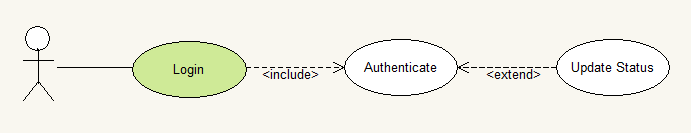
\includegraphics[width=6.0in, height=1.2in]{./loginCase.png}
					\\\caption{[Figure 1] Login Use Case}
			\end{figure*}\\
\newpage				
		\noindent \left\textbf{View Contact List}\\
		\begin{figure*}
					\centering
					\\ 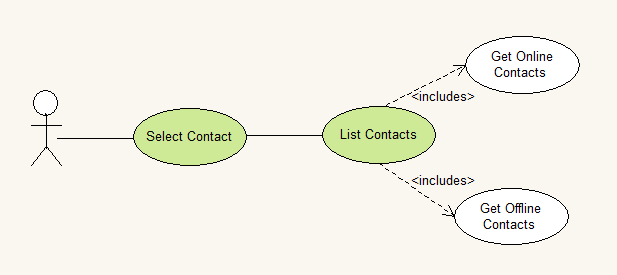
\includegraphics[width=6.0in, height=2.5in]{./viewContactsCase.png} \\
					\\\caption{[Figure 2] View Contact List Use Case} \\
		\end{figure*}\\ 
				
		\noindent \left\textbf{Messaging}\\
		\begin{figure*}
			\centering
			\\ 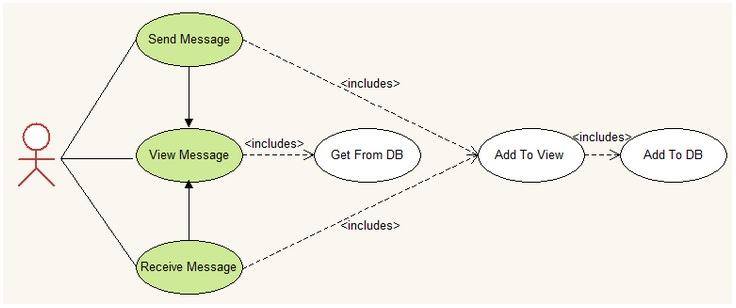
\includegraphics[width=6.0in, height=3.5in]{./messagingUseCase.jpg}
			\\\caption{[Figure 3] Messaging Use Case}\\
		\end{figure*}
\newpage		
		\noindent \left\textbf{Exit}\\
		\begin{figure*}
			\centering
			\\ 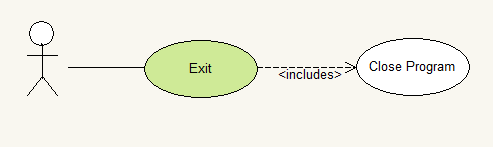
\includegraphics[width=6.0in, height=1.5in]{./exitCase.png}
			\\\caption{[Figure 4] Exit Use Case}\\
		\end{figure*}
\newpage	
	\noindent \\ \left\textbf{3.3 Class Diagram}\\
			\begin{figure*}
				\centering
				\\ 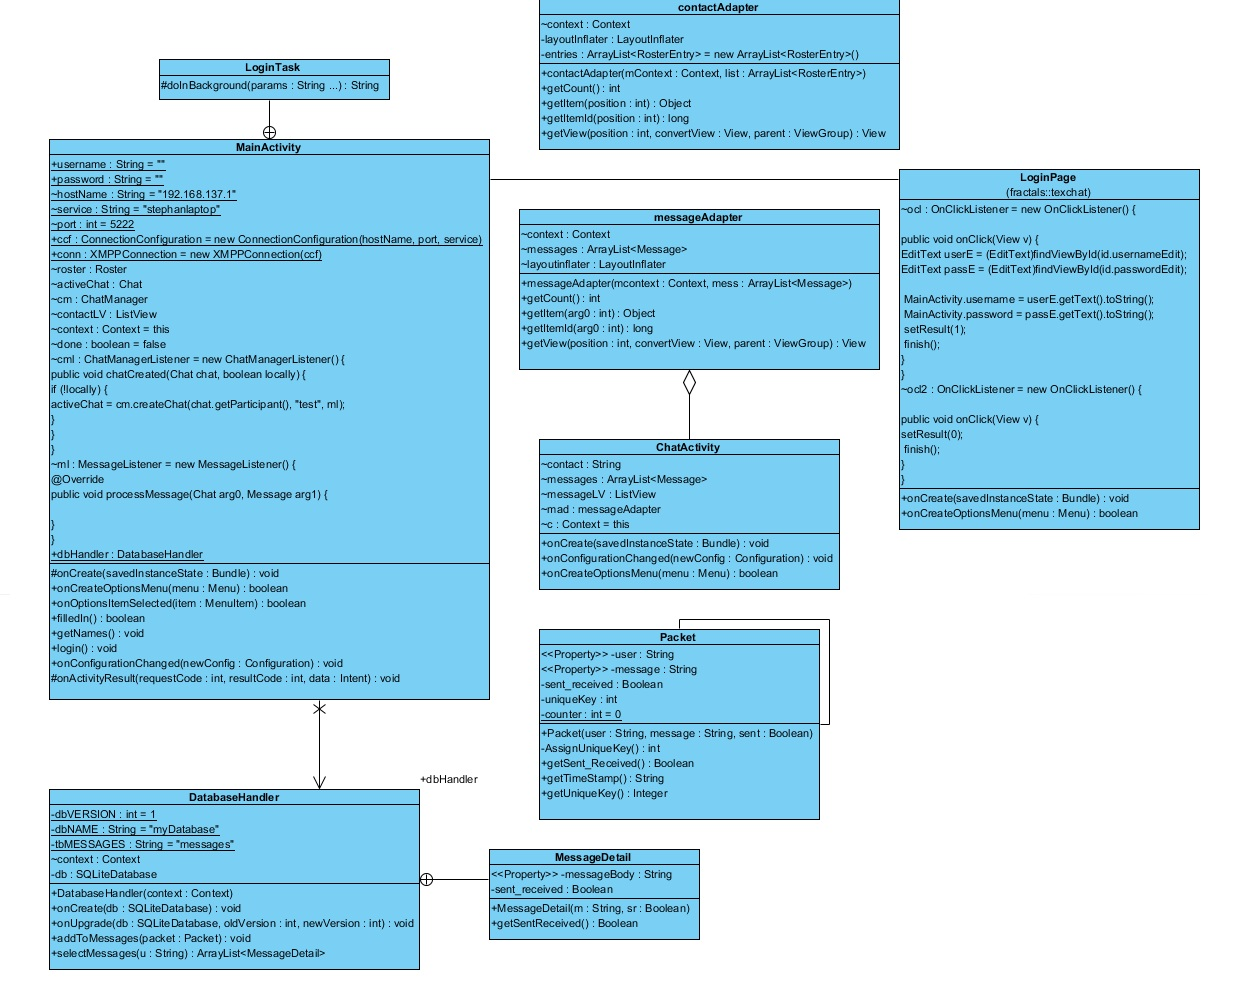
\includegraphics[width=7.0in, height=8.5in]{./Class_Diagram.jpg}
				\\\caption{[Figure 5] Class Diagram}\\
			\end{figure*}
	
	\\ \noindent \textbf{3.4 Entity Relationship Diagram}
	\\The system makes use of one SQLite database on the client side.  This database contains one table, namely Messages, that is used to record message histories for a particular client.  This release does not include any database cleanup components, and these may expected from later phases of development.\\ \\
	
	\begin{figure*}
		\centering
		\\ 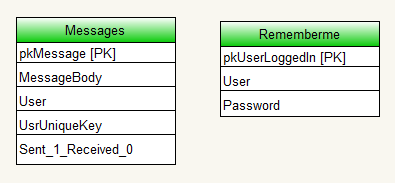
\includegraphics[width=3.0in, height=3.0in]{./erd.png}
		\\\caption{[Figure 6] ERD}\\
	\end{figure*}
	
\newpage	
	\section*{\textbf{4. External Interface Requirements}}
	\vspace{4mm}
		\begin{itemize}
			\item There is an external interface with the smack library.
			\item The mimeTeX library is also an external interface used within the application, the Native Development Kit acts as a bridge between Java and C/C++ when this library is used.
			\item The internal API uses the smack api to exchange the messages.
			\item The internal API is used to store data in the database on the device.
		\end{itemize}

\newpage	
		\section*{\textbf{5. Technical Requirements(Non-Functional)}}
		\vspace{4mm}
		\noindent \textbf{5.1 Non-Functional Requirements}\\
		
		\noindent \textbf{Authentication}\\
			Authentication happens server side. \\
			A login page is created to allow the user access to the application and its features. \\
			As soon as the user’s credentials has been authenticated he/she is logged into the application.\\
			
		\noindent \textbf{Authirozation}\\
		At this point there is no authorization yet.
		
		\noindent \textbf{Scalability}\\
		At this point in time the system is developed to handle only 2 users at a time. It will later be scaled upwards to handle a larger amount of concurrent users.\\
		
		
		\noindent \textbf{Audit-ability}\\
		The messages are logged on the phone’s database created by the application as soon as it is installed.\\
		
		\noindent \textbf{5.2 Technical Specification}\\
		Platforms to be supported:
		\begin{itemize}
			\item Android
		\end{itemize}
		Will use both Java and C. C will be used as native code.
		Is developed to communicate with a local server
		The database is handled with SQLite.\\
		
\newpage	
	\section*{\textbf{6. Open Issues}}
	\vspace{4mm}
		\begin{itemize}
			\item Understanding the MimeTeX library.
			\item Understanding how to render the LaTeX code using the MimeTeX library.
			\item Rendering the image inline (with the normal message text before it).
			
		\end{itemize}
	\vspace{5mm}

\newpage	
	\section*{\textbf{7. Glossary}}
	\vspace{4mm}
		\begin{itemize}
			\item SDK - Software Development Kit
			\item NDK - Native Development Kit
			\item ADT - Android Development Toolkit plugin
			\item IDE - Integrated Development Environment
			\item RUP - Rational Unified Process
			\item XML - eXtensible Markup Language
			\item Agile - Development methodology
			\item MVC - Model View Controller
			\item UML - Unified Modelling Language
			\item API - Application Programming Interface
			\item MimeTex - LaTeX library ported to Android
			\item C - Programming language.
			
		\end{itemize}
	\vspace{5mm}
\end{document}